\subsection{A Bivariate Joint Model for the Longitudinal PSA, and DRE Measurements, and Time of Cancer Progression}
Let $T_i^*$ denote the true cancer progression time of the ${i\mbox{-th}}$ patient included in PRIAS. Since biopsies are conducted periodically, $T_i^*$ is observed with interval censoring ${l_i < T_i^* \leq r_i}$. When progression is observed for the patient at his latest biopsy time $r_i$, then $l_i$ denotes the time of the second latest biopsy. Otherwise, $l_i$ denotes the time of the latest biopsy and ${r_i=\infty}$. Let $\boldsymbol{y}_{di}$ and $\boldsymbol{y}_{pi}$ denote his observed DRE and PSA longitudinal measurements, respectively. The observed data of all $n$ patients is denoted by ${\mathcal{D}_n = \{l_i, r_i, \boldsymbol{y}_{di}, \boldsymbol{y}_{pi}; i = 1, \ldots, n\}}$.

\begin{figure}[!htb]
\captionsetup{justification=justified}
\centerline{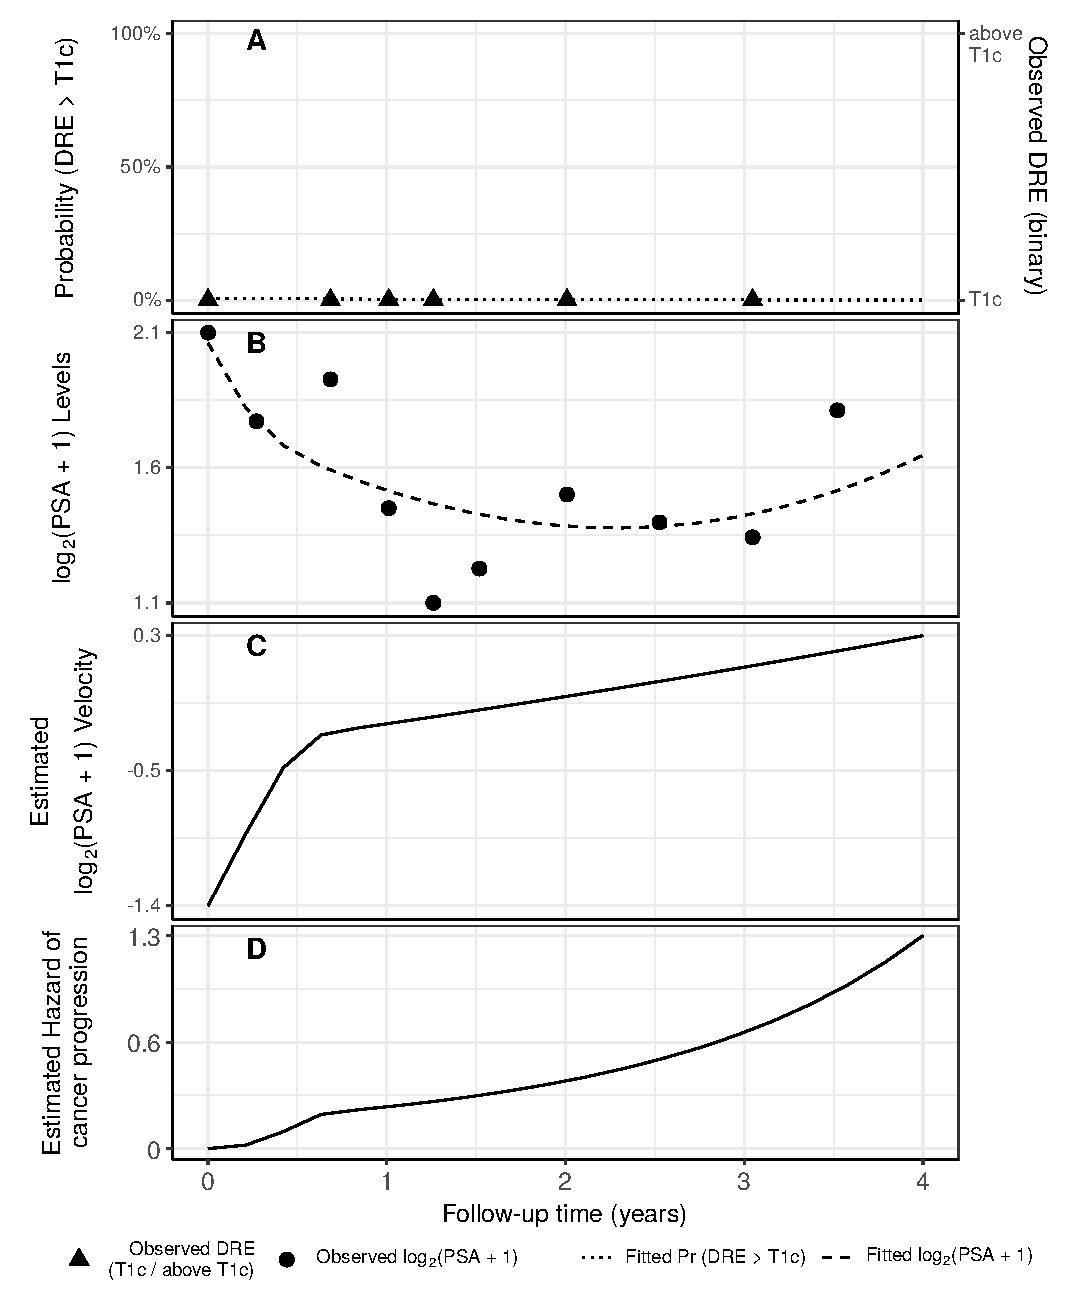
\includegraphics[width=\columnwidth]{images/jmExplanationPlot_1757.eps}}
\caption{\textbf{Illustration of the joint model fitted to the PRIAS dataset}. \textbf{Panel~A:} shows the observed DRE measurements and the fitted probability of obtaining $\mbox{DRE} > \mbox{T1c}$ (Equation~\ref{eq:long_model_dre}) for $i$-th patient. \textbf{Panel~B:} shows the observed and fitted $\log_2(\mbox{PSA} + 1)$ measurements (Equation~\ref{eq:long_model_psa}). \textbf{Panel~C:} shows the estimated $\log_2(\mbox{PSA} + 1)$ velocity (velocity cannot be observed directly) over time. The hazard function (Equation~\ref{eq:rel_risk_model}) shown in \textbf{Panel~D}, depends on the fitted log odds of having a $\mbox{DRE} > \mbox{T1c}$, and the fitted $\log_2(\mbox{PSA} + 1)$ value and velocity.}
\label{fig:jmExplanationPlot_1757}
\end{figure}

In our joint model, the patient-specific DRE and PSA measurements over time are modeled using a bivariate generalized linear mixed effects sub-model. The sub-model for DRE is given by (see~Panel~A, Figure~\ref{fig:jmExplanationPlot_1757}):
\begin{equation}
\label{eq:long_model_dre}
\begin{split}
    \mbox{logit} \big[\mbox{Pr}\{y_{di}(t) > \mbox{T1c}\}\big] &= \beta_{0d} + b_{0di} + (\beta_{1d} + b_{1di}) t\\
    &+ \beta_{2d} (\mbox{Age}_i-70) + \beta_{3d} (\mbox{Age}_i-70)^2
    \end{split}
\end{equation}
where, $t$ denotes the follow-up visit time, and $\mbox{Age}_i$ is the age of the ${i\mbox{-th}}$ patient at the time of inclusion in AS. We have centered the Age variable around the median age of 70 years for better convergence during parameter estimation. However, this does not change the interpretation of the parameters corresponding to the Age variable. The fixed effect parameters are denoted by ${\{\beta_{0d}, \ldots, \beta_{3d}\}}$, and ${\{b_{0di}, b_{1di}\}}$ are the patient specific random effects. With this definition, we assume that the patient-specific log odds of obtaining a DRE measurement larger than T1c remain linear over time. 

The mixed effects sub-model for PSA is given by (see~Panel~B, Figure~\ref{fig:jmExplanationPlot_1757}):
\begin{equation}
\label{eq:long_model_psa}
\begin{split}
    \log_2 \big\{y_{pi}(t) + 1\big\} &= m_{pi}(t) + \varepsilon_{pi}(t),\\
    m_{pi}(t) &= \beta_{0p} + b_{0pi} + \sum_{k=1}^4 (\beta_{kp} + b_{kpi})  B_k(t,\mathcal{K})\\ 
    &+ \beta_{5p} (\mbox{Age}_i-70) + \beta_{6p} (\mbox{Age}_i-70)^2,
    \end{split}
\end{equation}
where, $m_{pi}(t)$ denotes the underlying measurement error free value of $\log_2 (\mbox{PSA} + 1)$ transformed \citep{pearson1994mixed,lin2000latent} measurements at time $t$. We model it non-linearly over time using B-splines \citep{de1978practical}. To this end, our B-spline basis function $B_k(t, \mathcal{K})$ has 3 internal knots at $\mathcal{K} = \{0.1, 0.7, 4\}$ years, and boundary knots at 0 and 5.42 years (95-th percentile of the observed follow-up times). This specification allows fitting the $\log_2 (\mbox{PSA} + 1)$ levels in a piecewise manner for each patient separately. The internal and boundary knots specify the different time periods (analogously pieces) of this piecewise curve. The fixed effect parameters are denoted by ${\{\beta_{0p},\ldots,\beta_{6p}\}}$, and ${\{b_{0pi}, \ldots, b_{4pi}\}}$ are the patient specific random effects. The error $\varepsilon_{pi}(t)$ is assumed to be t-distributed with three degrees of freedom (see~Appendix~B.1) and scale $\sigma$, and is independent of the random effects. 

To account for the correlation between the DRE and PSA measurements of a patient, we link their corresponding random effects. More specifically, the complete vector of random effects ${\boldsymbol{b}_i = (b_{0di}, b_{1di}, b_{0pi}, \ldots, b_{4pi})^T}$ is assumed to follow a multivariate normal distribution with mean zero and variance-covariance matrix $\boldsymbol{D}$.

To model the impact of DRE and PSA measurements on the risk of cancer progression, our joint model uses a relative risk sub-model. More specifically, the hazard of cancer progression $h_i(t)$ at a time $t$ is given by (see~Panel~D, Figure~\ref{fig:jmExplanationPlot_1757}):
\begin{equation}
\label{eq:rel_risk_model}
\begin{split}
    h_i(t) &= h_0(t) \exp\Big(\gamma_1 (\mbox{Age}_i-70) + \gamma_2 (\mbox{Age}_i-70)^2\\
    &+\alpha_{1d} \mbox{logit} \big[\mbox{Pr}\{y_{di}(t) > \mbox{T1c}\}\big]+ \alpha_{1p} m_{pi}(t) + \alpha_{2p} \frac{\partial m_{pi}(t)}{\partial {t}}\Big),
    \end{split}
\end{equation}
where, $\gamma_1, \gamma_2$ are the parameters for the effect of age. The parameter $\alpha_{1d}$ models the impact of log odds of obtaining a $\mbox{DRE} > \mbox{T1c}$ on the hazard of cancer progression. The impact of PSA on the hazard of cancer progression is modeled in two ways: a) the impact of the error free underlying PSA value $m_{pi}(t)$ (see~Panel~B, Figure~\ref{fig:jmExplanationPlot_1757}), and b) the impact of the underlying PSA velocity $\partial m_{pi}(t)/\partial {t}$ (see~Panel~C, Figure~\ref{fig:jmExplanationPlot_1757}). The corresponding parameters are $\alpha_{1p}$ and $\alpha_{2p}$, respectively. Lastly, $h_0(t)$ is the baseline hazard at time $t$, and is modeled flexibly using P-splines \citep{eilers1996flexible}. The detailed specification of the baseline hazard $h_0(t)$, and the joint parameter estimation of the two sub-models using the Bayesian approach (R package \textbf{JMbayes}\cite{rizopoulosJMbayes}) are presented in Appendix A of the supplementary material.
